% Choose one to switch between slides and handout
%\documentclass[]{beamer}
\documentclass[handout]{beamer}

% Video Meta Data
\title{Bitcoin, Blockchain and Cryptoassets}
\subtitle{Risks \& Illicit Activity}
\author{Prof. Dr. Fabian Schär}
\institute{University of Basel}

% Config File
% Packages
\usepackage[utf8]{inputenc}
\usepackage{hyperref}
\usepackage{gitinfo2}
\usepackage{tikz}
\usepackage{amsmath}
\usepackage{mathtools}
\usepackage{bibentry}
\usepackage{xcolor}
\usepackage{colortbl} % Add colour to LaTeX tables
\usepackage{caption}
\usepackage[export]{adjustbox}
\usepackage{pgfplots} \pgfplotsset{compat = 1.17}
\usepackage{makecell}
\usepackage{fancybox}
\usepackage{ragged2e}
\usepackage{fontawesome}
\usepackage{seqsplit}
\usepackage{tabularx}

% Color Options
\definecolor{highlight}{rgb}{0.65,0.84,0.82}
\definecolor{focus}{rgb}{0.72, 0, 0}
\definecolor{lightred}{rgb}{0.8,0.5,0.5}
\definecolor{midgray}{RGB}{190,195,200}

% Beamer Template Options
\beamertemplatenavigationsymbolsempty
\setbeamertemplate{footline}[frame number]
\setbeamercolor{structure}{fg=black}
\setbeamercolor{footline}{fg=black}
\setbeamercolor{title}{fg=black}
\setbeamercolor{frametitle}{fg=black}
\setbeamercolor{item}{fg=black}
\setbeamercolor{}{fg=black}
\setbeamercolor{bibliography item}{fg=black}
\setbeamercolor*{bibliography entry title}{fg=black}
\setbeamercolor{alerted text}{fg=focus}
\setbeamertemplate{items}[square]
\setbeamertemplate{enumerate items}[default]
\captionsetup[figure]{labelfont={color=black},font={color=black}}
\captionsetup[table]{labelfont={color=black},font={color=black}}

\setbeamertemplate{bibliography item}{\insertbiblabel}

% Link Icon Command
\newcommand{\link}{%
    \tikz[x=1.2ex, y=1.2ex, baseline=-0.05ex]{%
        \begin{scope}[x=1ex, y=1ex]
            \clip (-0.1,-0.1)
                --++ (-0, 1.2)
                --++ (0.6, 0)
                --++ (0, -0.6)
                --++ (0.6, 0)
                --++ (0, -1);
            \path[draw,
                line width = 0.5,
                rounded corners=0.5]
                (0,0) rectangle (1,1);
        \end{scope}
        \path[draw, line width = 0.5] (0.5, 0.5)
            -- (1, 1);
        \path[draw, line width = 0.5] (0.6, 1)
            -- (1, 1) -- (1, 0.6);
        }
    }

% Read Git Data from Github Actions Workflow
% Defaults to gitinfo2 for local builds
\IfFileExists{gitInfo.txt}
	{\input{gitInfo.txt}}
	{
		\newcommand{\gitRelease}{(Local Release)}
		\newcommand{\gitSHA}{\gitHash}
		\newcommand{\gitDate}{\gitAuthorIsoDate}
	}

% Custom Titlepage
\defbeamertemplate*{title page}{customized}[1][]
{
  \vspace{-0cm}\hfill\includegraphics[width=2.5cm]{../config/logo_cif}
  \includegraphics[width=1.9cm]{../config/seal_wwz}
  \\ \vspace{2em}
  \usebeamerfont{title}\textbf{\inserttitle}\par
  \usebeamerfont{title}\usebeamercolor[fg]{title}\insertsubtitle\par  \vspace{1.5em}
  \small\usebeamerfont{author}\insertauthor\par
  \usebeamerfont{author}\insertinstitute\par \vspace{2em}
  \usebeamercolor[fg]{titlegraphic}\inserttitlegraphic
    \tiny \noindent \texttt{Release Ver.: \gitRelease}\\ 
    \texttt{Version Hash: \gitSHA}\\
    \texttt{Version Date: \gitDate}\\ \vspace{1em}
    
    
    \iffalse
  \link \href{https://github.com/cifunibas/Bitcoin-Blockchain-Cryptoassets/blob/main/slides/intro.pdf}
  {Get most recent version}\\
  \link \href{https://github.com/cifunibas/Bitcoin-Blockchain-Cryptoassets/blob/main/slides/intro.pdf}
  {Watch video lecture}\\ 
  
  \fi
  
  \vspace{1em}
  License: \texttt{Creative Commons Attribution-NonCommercial-ShareAlike 4.0 International}\\\vspace{2em}
  \includegraphics[width = 1.2cm]{../config/license}
}


% tikzlibraries
\usetikzlibrary{decorations.pathreplacing}
\usetikzlibrary{decorations.markings}
\usetikzlibrary{positioning}
\usetikzlibrary{calc}
\captionsetup{font=footnotesize}


%%%%%%%%%%%%%%%%%%%%%%%%%%%%%%%%%%%%%%%%%%%%%%
%%%%%%%%%%%%%%%%%%%%%%%%%%%%%%%%%%%%%%%%%%%%%%
\begin{document}

\thispagestyle{empty}
\begin{frame}[noframenumbering]
	\titlepage
\end{frame}


%%%
\begin{frame}{Quantifying Illicit Activity}
	Illicit activities with cryptocurrencies pose a certain problem but are hard to quantify. \\
	\vspace{1em}
	Number of users or transactions are flawed measurables:
		\begin{itemize}
			\item One user $\rightarrow$ Multiple addresses
			\item Multiple Users $\rightarrow$ One address
			\item Transaction $\neq$ Transaction
			\item Obfuscation transactions
		\end{itemize}
	\vspace{1em} 
	Studies use different assumptions in order to carry out estimates, which can have a big influence on the results.	
\end{frame}
%%%	


%%%
\begin{frame}{Origin and Homogenity of Bitcoin Units}
	Each output has a clearly distinguishable origin.
	\begin{figure}
		\resizebox{10cm}{6cm}{
			\begin{tikzpicture}[
     		 roundnode1/.style = {circle,  draw=highlight, fill=highlight!5},
     		 roundnode2/.style = {circle,  draw=focus!50, fill=focus!5},
      		squarednode/.style = {rectangle, draw=black!60, fill=black!5},
     		 ]
			
    \node[roundnode2]    (nodeA)                                    {\texttt{A}};
    \node[roundnode2]    (nodeB)        [below=8mm of nodeA]        {\texttt{B}};
    \node[roundnode2]    (nodeC)        [below=8mm of nodeB]        {\texttt{C}};
    \node[roundnode2]    (nodeD)        [below=8mm of nodeC]        {
\includegraphics[scale=0.025]{../assets/images/agents/intermediary_devil}};
    \node[roundnode2]    (nodeE)        [below=10mm of nodeD]       {\texttt{E}};
    
    \node[squarednode]  (TRX1)          [right =of nodeA]           {\texttt{TRX1}}; 
    \node[squarednode]  (TRX2)          [below =17mm of TRX1]       {\texttt{TRX2}};
    \node[squarednode]  (TRX3)          [right =8mm of nodeD]      {\texttt{TRX3}};
    \node[squarednode]  (TRX4)          [right =of nodeE]           {\texttt{TRX4}};
    
    \node[roundnode2]    (nodeF)        [right =of TRX1]            {\texttt{F}};
    \node[roundnode2]    (nodeG)        [right =of TRX2]            {\texttt{G}};
    \node[roundnode2]    (nodeI)        [right =of TRX3]            {\texttt{I}};
    \node[roundnode2]    (nodeH)        [above =4mm of nodeI]       {\texttt{H}};
    \node[roundnode2]    (nodeJ)        [below =2mm of nodeI]       {\texttt{J}};
    \node[roundnode2]    (nodeK)        [right =of TRX4]            {\texttt{K}};
    
    \node[squarednode]  (TRX5)          [right =of nodeF]          {\texttt{TRX5}}; 
    \node[squarednode]  (TRX6)          [right =of nodeG]          {\texttt{TRX6}};
    \node[squarednode]  (TRX7)          [right =of nodeK]          {\texttt{TRX7}};
    
    \node[roundnode1]    (nodeO)        [right =of TRX6]            {\texttt{O}};
    \node[roundnode2]    (nodeN)        [above =3mm of nodeO]       {\texttt{N}};
    \node[roundnode2]    (nodeM)        [above =3mm of nodeN]       {\texttt{M}};
    \node[roundnode1]    (nodeL)        [above =1mm of nodeM]       {\texttt{L}};
    \node[roundnode2]    (nodeP)        [below =4mm of nodeO]       {\texttt{P}};
    \node[roundnode2]    (nodeQ)        [right =of TRX7]            {\texttt{Q}};
    
    \node[squarednode]  (TRX9)          [right = 48mm of nodeI]    {\texttt{TRX9}};
    \node[squarednode]  (TRX8)          [above = 33mm of TRX9]     {\texttt{TRX8}};
    
    \node[roundnode1]    (nodeS)        [right =of TRX8]            {\texttt{S}};
    \node[roundnode1]    (nodeR)        [above =2mm of nodeS]       {\texttt{R}};
    \node[roundnode1]    (nodeT)        [below =2mm of nodeS]       {\texttt{T}};
    \node[roundnode1]    (nodeU)        [right =of TRX9]            {\texttt{U}};
    
    
    \draw[-] (nodeA) -- (TRX1);
    \draw[-] (nodeB) -- (TRX2);
    \draw[-] (nodeC) -- (TRX2);
    \draw[-] (nodeD) -- (TRX3);
    \draw[-] (nodeE) -- (TRX4);
    
    \draw[-] (TRX1) -- (nodeF);
    \draw[-] (TRX2) -- (nodeG);
    \draw[-] (TRX3) -- (nodeH);
    \draw[-] (TRX3) -- (nodeI);
    \draw[-] (TRX3) -- (nodeJ);
    \draw[-] (TRX4) -- (nodeK);
    
    \draw[-] (nodeF) -- (TRX5);
    \draw[-] (nodeG) -- (TRX6);
    \draw[-] (nodeH) -- (TRX6);
    \draw[-] (nodeJ) -- (TRX7);
    \draw[-] (nodeK) -- (TRX7);
    
    \draw[-] (TRX5) -- (nodeL);
    \draw[-] (TRX5) -- (nodeM);
    \draw[-] (TRX6) -- (nodeN);
    \draw[-] (TRX6) -- (nodeO);
    \draw[-] (TRX6) -- (nodeP);
    \draw[-] (TRX7) -- (nodeQ);
    
    \draw[-] (nodeM) -- (TRX8);
    \draw[-] (nodeN) -- (TRX8);
    \draw[-] (nodeP) -- (TRX9);
    \draw[-] (nodeQ) -- (TRX9);
    \draw[-] (nodeI) -- (TRX9);
    
    \draw[-] (TRX8) -- (nodeR);
    \draw[-] (TRX8) -- (nodeS);
    \draw[-] (TRX8) -- (nodeT);
    \draw[-] (TRX9) -- (nodeU);
 
			\end{tikzpicture}
		}
	\end{figure}	
\end{frame}
%%%


%%%
\begin{frame}{Silk Road}
	\begin{itemize}
		\item First modern large-scale darknet market
		\item Trading of illegal drugs and digital goods
		\item Bitcoin as dominant medium of exchange
	\end{itemize}
	\vspace{1em}
	\centering
	\begin{tikzpicture}[squarednode/.style = {rectangle, draw=black!60, fill=black!5}]
		\node (AgentSeller)				{
\includegraphics[scale=0.05]{../assets/images/agents/handing_right}};
		\node (Seller)	[below= 0.05cm of AgentSeller]			{Seller};
	
		\node (Darknet)          [right = 2cm of AgentSeller]          {
\includegraphics[scale=0.1]{../assets/images/darknet}}; 
		\node (Silkroad)	[below= 0.05cm of Darknet]			{Silkroad};
	
		\node (AgentBuyer)		[right =2cm of Darknet]		{
\includegraphics[scale=0.05]{../assets/images/agents/handing_money_left}};
		\node (Buyer)	[below= 0.05cm of AgentBuyer]			{Buyer};
	
		\draw[->, thick] (AgentBuyer) edge [out=-230, in=50] node[midway,above] {\texttt{BTC}} (Darknet);
		\draw[->, thick, dotted] (Darknet) edge [out=-230, in=50] node[midway,above] {\texttt{BTC}} (AgentSeller);
		\draw[->, thick] (AgentSeller) edge [out=-45, in=-140] node[midway,below] {\texttt{Good}} (AgentBuyer);
	\end{tikzpicture}
\end{frame}
%%%


%%%
\begin{frame}{Mt. Gox}
	\centering
		\begin{itemize}
			\item Worlds largest bitcoin exchange in 2013.
			\item Transaction malleability as reason for stopping Bitcoin withdrawals in February 2014.
			\item Mistake: Relied solely on the transaction hash to track and verify its account balance.
			\item Claim that transaction malleability as the reason for the loss of around 850'000 is controversial. See \cite{Decker2014}
		\end{itemize}
	
\includegraphics[scale=0.12]{../assets/images/mt_gox}\\
	\footnotesize{Picture source: Wikipedia}	
\end{frame}
%%%


%%%
\begin{frame}{Malleability Attack}
	\centering
	\begin{tikzpicture}[squarednode/.style = {rectangle, draw=black!60, fill=black!5}]
		%User
	\node (AvatarUser) at (0,0.5)	{
\includegraphics[scale=0.04]{../assets/images/agents/agent_right}};
	\node (User)[below= 0.05cm of AvatarUser]{{\scriptsize User}};
		
%Mt.Gox
	\node (CEX)	at (4,0.5){
\includegraphics[scale=0.04]{../assets/images/agents/handing_money_left}};
	\node (Mt.Gox)[below= 0.05cm of CEX]{{\scriptsize Mt.Gox}};
				
%Network
	\node at (1.5,5) {\scriptsize Bitcoin Network};  
	\node (agenta) at (-2,3.8) {\includegraphics[width = 0.5 cm]{../assets/images/agents/avatar_rand3.png}};
	\node (agentb) at (-1,2.5) {\includegraphics[width = 0.5 cm]{../assets/images/agents/avatar_rand4.png}};
	\node (agentc) at (0,4.2) {\includegraphics[width = 0.5 cm]{../assets/images/agents/avatar_rand5.png}};
	\node (agentd) at (2.5,3.8) {\includegraphics[width = 0.5 cm]{../assets/images/agents/avatar_rand1.png}};
	\node (agente) at (1,2.6) {\includegraphics[width = 0.5 cm]{../assets/images/agents/avatar_rand2.png}};	
	\node (agentf) at (4.5,4.5) {\includegraphics[width = 0.5 cm]{../assets/images/agents/avatar_rand2.png}};	
	\node (agentg) at (3,2.3) {\includegraphics[width = 0.5 cm]{../assets/images/agents/avatar_rand2.png}};
	\node (agenth) at (5,2.7) {\includegraphics[width = 0.5 cm]{../assets/images/agents/avatar_rand2.png}};		
	
%Connection
	\only<1->{
		\draw[->, thick, dotted](AvatarUser) edge [out=-30, in=-150] node[midway,below] {{\tiny Withdrawal Request}} (CEX);
		}
	\only<2->{	
		\draw[->, thick, dotted] (CEX) edge [out=-210, in=30] node[midway,above] {{\tiny $TXID_{a}$}} (AvatarUser);
		\draw[->, thick, dotted] 	(CEX) -- (agenth.south) node[midway] {\scriptsize $TXID_{a}$};
		}

%Peer connections
	\only<3->{
	\draw[->, thick ,dotted]	(AvatarUser.north) -- (agentb.south) node[midway] {\color{red}\scriptsize $TXID_{m}$};
		}
	
	\draw[-]	(agenta) -- (agentc);
	\draw[-]	(agenta) -- (agentb);
	
	\draw[-]	(agentb) -- (agentc);
	\draw[-]	(agentb) -- (agente);
	

	\draw[-]	(agentc) -- (agentd);
	\draw[-]	(agentc) -- (agente);
	
	\draw[-]	(agentd) -- (agente);
	\draw[-]	(agentd) -- (agentf);
	\draw[-]	(agentd) -- (agenth);

	\draw[-]	(agente) -- (agentg);

	\draw[-]	(agentf) -- (agenth);
	
	\draw[-]	(agentg) -- (agenth);
	\end{tikzpicture}
	\begin{enumerate}
	\setcounter{enumi}{2}
		\item<3-> User modifies $TRX_{a}$ by altering the scriptSig without invalidating it. Modification results in a different transaction ID ($TXID_{b}$).
		\item<4-> Modified $TRX_{b}$ races with original $TXR_{a}$ for confirmation.
		\item<5-> If modified version gets included in the blockchain:
		\begin{itemize}
			\item User still receives BTC units.
			\item Mt. Gox thinks $TRX_{a}$ failed, as they only check for $TXID_{a}$. User still credited with funds in their system.
		\end{itemize}
	\end{enumerate}
\end{frame}
%%%


%%%
\begin{frame}{Wannacry}
	\centering
		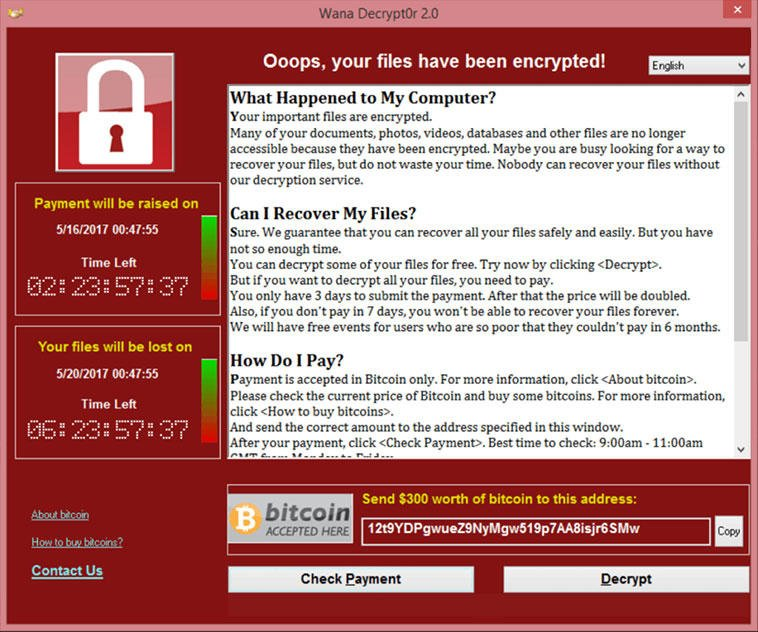
\includegraphics[scale=0.28]{../assets/images/wannacry} \\
		\footnotesize{Picture source: OneSpan Blog}\\
		\vspace{1em}
		\begin{small}
			\texttt{13AM4VW2dhxYgXeQepoHkHSQuy6NgaEb94} \link \href{https://blockstream.info/address/13AM4VW2dhxYgXeQepoHkHSQuy6NgaEb94}{} \\
			\texttt{12t9YDPgwueZ9NyMgw519p7AA8isjr6SMw} \link \href{https://blockstream.info/address/12t9YDPgwueZ9NyMgw519p7AA8isjr6SMw}{} \\
			\texttt{115p7UMMngoj1pMvkpHijcRdfJNXj6LrLn} \link \href{https://blockstream.info/address/115p7UMMngoj1pMvkpHijcRdfJNXj6LrLn} {} \\
		\end{small}
\end{frame}
%%%


%%%
\begin{frame}{Other Risks \& Illicit Activities}
	\textbf{Botnet Miner}
		\begin{itemize}
			\item Malware that integrates a victims computer into the "botnet".
			\item Compromised computers can be used for mining.
		\begin{center}
		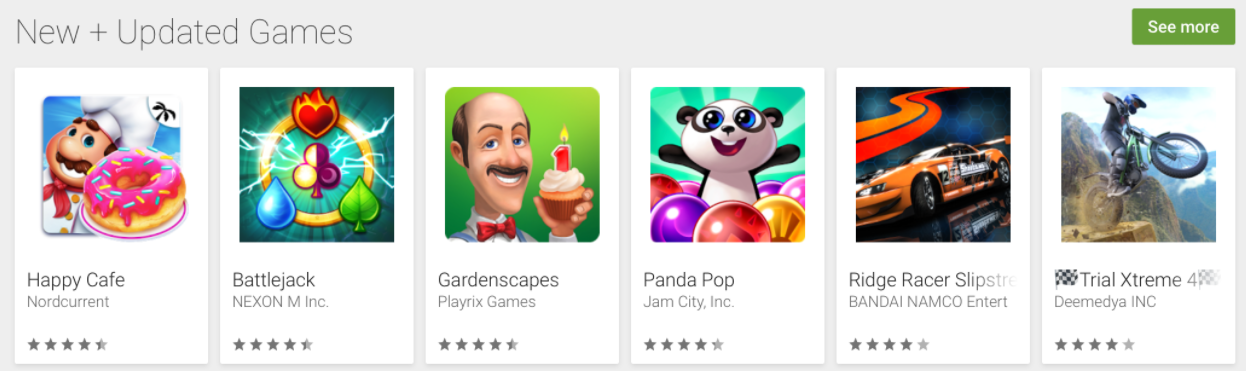
\includegraphics[scale=0.25]{../assets/images/google_playstore}\\
		\footnotesize{Picture source: Google}
		\end{center}
		\end{itemize}
	%\vspace{1em}
	\textbf{Bitcoin Tumbler}
		\begin{itemize}
			\item Used to disguise the origin of Bitcoin units and links between old and new addresses.
			\item How: Send coins from users around, Randomize transaction amounts, Add time delays
		\end{itemize}	
\end{frame}
%%%


%%%
\begin{frame}{Regulation}
	Bitcoin Network because of decentralized nature hard to regulate $\rightarrow$ Focus on On- and Off-ramps\\
	\vspace{1em}
	Example: {\color{focus} OpenVASP } (Virtual asset service providers)
		\begin{itemize}
			\item Protocol facilitating compliance with global travel rule requirements for VASPs. Shared communication protocol to exchange VA transfer information.
		\end{itemize}
	\vspace{1em}
	\textbf{Because of the high transparency, Bitcoin is not very suitable for usage with illegal activities.}
\end{frame}
%%%

\begin{frame}%[allowframebreaks]
\frametitle{References and Recommended Reading}
	\bibliographystyle{amsplain}
	\bibliography{../assets/bib/refs}
\end{frame}


\end{document}